
\section{The Virtual Closed-Loop Prosthesis}

In order to test the usability of the two sensory feedback configurations in a closed-loop control system, a prosthesis which accommodates this had to be developed. As no commercial or research prostheses were available in this project, a virtual system resembling prosthetic control was made. \\
The aim was to develop a system which could provide control and feedback of two degrees of freedom. For this purpose, it was chosen to incorporate the rotational degree of freedom in wrist supination and pronation and a grasp degree of freedom in open and closed hand. In \figref{fig:meth:gridmap} is a depiction of a grid and a cursor dot symbolizing the different possible prosthetic states and the current prosthetic state, respectively. Performing supination would make the cursor move to the right into one of two possible states, while performing pronation would make the cursor move left into one of two states. Performing the closed hand movement would make the cursor move downwards into one of four possible states and performing open hand would make the cursor move upwards. In total, the prosthesis could achieve a total of 25 different states, by performing single DoF movements or by combinations of two DoF's. However, it would only be possible to move the cursor in DoF at a time. In each of the squares, a unique electrotactile feedback was provided in each of the two feedback configurations, which will be further explained in the later \secref{sec:feed}.      
     

\begin{figure}[H]                 
	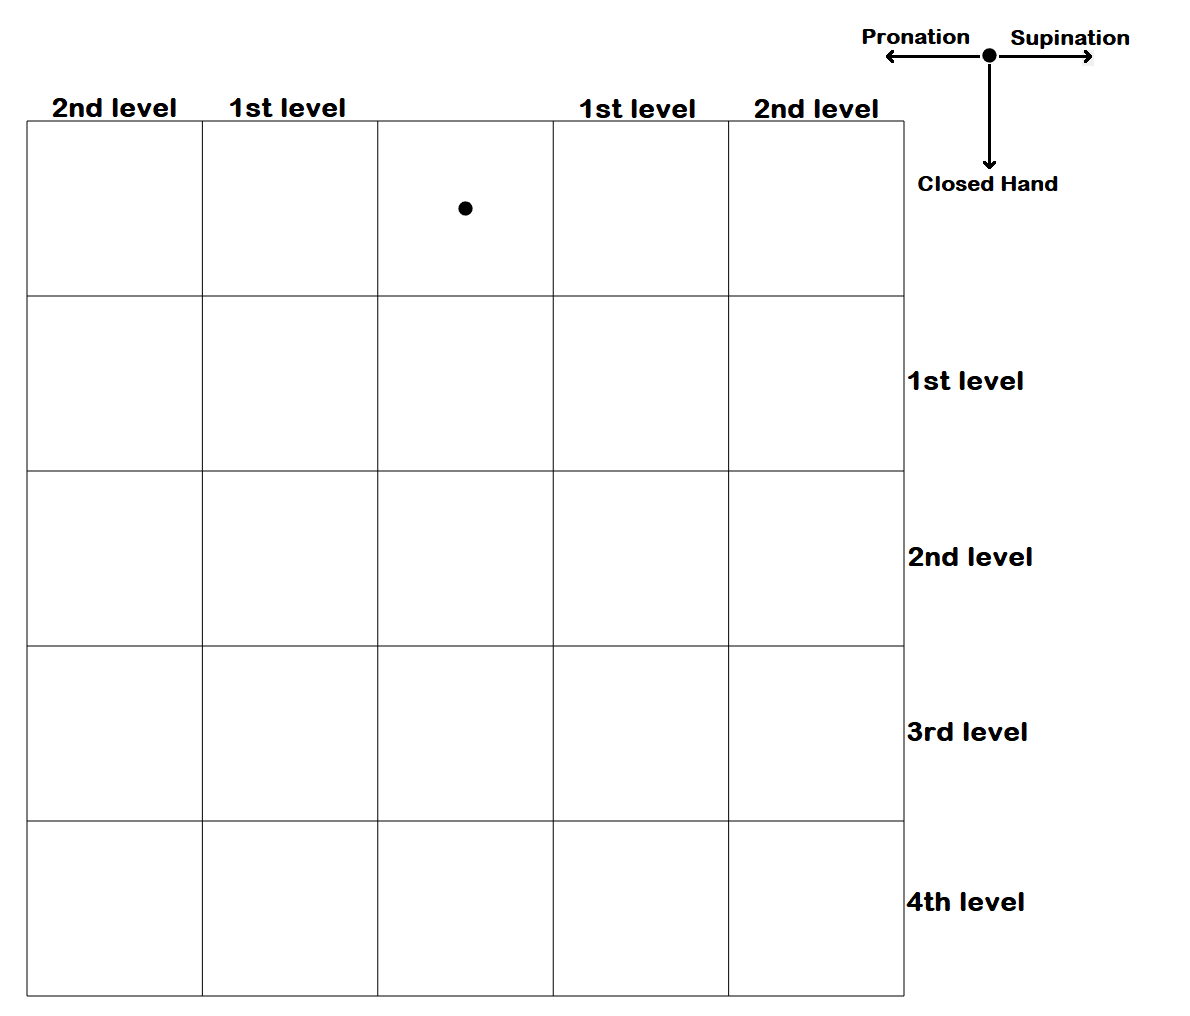
\includegraphics[width=0.9\textwidth]{figures/gridmap2}  
	\caption{Image of the grid map and cursor used in the experiment. Performing supination moves the cursor the right, pronation moves it to the left and closing the hand moves it down. Opening the hand moves the cursor up, and is used as a correction movement if a wrong movement has been made.}
	\label{fig:meth:gridmap} 
\end{figure}
%hand movements used 

%The Grid 